\chapter{Resultados e Discussão} \label{cap:resultados}

Neste capítulo apresentamos e analisamos os dados dos experimentos realizados com as configurações de rede propostas. Na seção \ref{sec:parcial} analisamos o comportamento das arquiteturas durante as épocas iniciais. Na seção \ref{sec:completo}, a configuração de rede escolhida é apresentada e sua performance comparada com o trabalho de referência. Na última seção apresentamos nossas discussão sobre a eficácia do método proposto.

\section{Experimentos Preliminares}\label{sec:parcial}

Como descrito no capítulo \ref{cap:modelagem}, as configurações propostas foram treinadas durante as 10 primeiras épocas para os valores de $l_r$ = $10^{-\eta}$, com $\eta=1,2,3,4,5$. Na tabela \ref{tab:modelos_iniciais} vemos o tamanho, o tempo médio na fase de treino e o tempo médio total por época de algumas das configurações propostas. O desvio padrão relativo é menor do que $0.1\%$ em todas as médias. Em geral, a etapa de treino constitui de $70\%$ a $85\%$ do tempo total de uma época.

\begin{table}[ht]
	\begin{center}
		\caption{Comparação do tempo de treino entre as arquiteturas.}
		\label{tab:modelos_iniciais}
		\begin{tabular}{ |c|c|c|c| }
			\hline
			modelo & 
			\begin{tabular}[c]{@{}c@{}}tamanho\\ (parâmetros)\end{tabular} & \begin{tabular}[c]{@{}c@{}}$\tilde{\tau}$\\(segundos) \end{tabular}& \begin{tabular}[c]{@{}c@{}}$\tau$\\ (segundos)\end{tabular}\\ \hline\hline
			% RMch
			(a) $M$ & $5.4\,10^{6}$  & $72.63$ & $100.97$ \\ \hline
			
			% RMchD
			(b) $MD$ & $5.4\,10^{6}$ & $75.96$ & $108.14$ \\ \hline
			
			% C5o6RMch
			(c) $C_6M$ & $2.4\,10^{6}$ & $66.96$ & $91.24$ \\ \hline
			
			% C5o6RMchD
			(d) $C_6MD$ & $2.4\,10^{6}$ & $71.19$ & $97.57$ \\ \hline
			
			% C5o6C5o12RMchD
			(e) $C_6C_{12}MD$ & $4.4\,10^{6}$ & $238.66$ & $291.03$ \\ \hline
			
			% C5o6C5o12Rfl100MchD
			(f) $C_6C_{12}Fl_{100}MD$ & $2.4\,10^{6}$ & $311.42$ & $357.51$ \\ \hline
			
			% C5o6C5o12C5o36C5o36RMchD
			(g) $C_6C_{12}C_{36}C_{36}MD$ & $4.5\,10^{5}$ & $249.53$ & $302.44$ \\ \hline
			
			% C5o6C5o12C5o36C5o36Rfl100MchD
			(h) $C_6C_{12}C_{36}C_{36}Fl_{100}MD$ & $2.9\,10^{5}$ & $256.97$ & $308.77$ \\ \hline
		\end{tabular}\hfill%
	\end{center}
\end{table}

A partir da tabela podemos ver que o tempo consumido para o treino de uma configuração depende não apenas da quantidade de parâmetros, mas também da arquitetura. As arquiteturas $C_6M$ e $C_6C_{12}Fl_{100}MD$, por exemplo, possuem aproximadamente o mesmo número de parâmetros, sendo a última, entretanto, pelo menos quatro vezes mais lenta. Em todas as configurações estudadas, a adição do dropout aumentou ligeiramente o tempo de treino (entre $4\%$ e $19\%$), mostrando-se uma operação computacionalmente barata. Operações de maxpooling (ver apêndice \ref{cap:apendice_arquiteturas}), entretanto, mostraram-se computacionalmente custosas, aumentando a demanda de tempo em mais de duas vezes para algumas arquiteturas. Chamamos a atenção para o fato de que a relação entre as camadas é tão importante para o tamanho e tempo de execução quanto a especificação da camada em sí. No par (d)-(e), por exemplo, a adição de uma camada convolucional aumentou consideravelmente o tamanho e o tempo de execução. Nesse caso, os canais extras adicionados aumentaram substancialmente o número de sinais de entrada na camada densa seguinte. No par (e)-(f), por outro lado, a camada densa reduz drasticamente a quantidade de sinais (de 24192 para 100), reduzindo o tamanho da entrada da camada multi-caractere seguinte, adicionando, entretanto, uma maior de demanda de tempo. Em geral, podemos estabelecer que camadas densas normalmente demandam mais tempo, enquanto camadas convolucionais, usualmente reduzem o número de sinais e tamanho total da arquitetura, mas o impacto exato precisa ser estimado em concordância demais camadas. Para comparação, o modelo no estudo de Pinto\cite{otaro} possui, aproximadamente, $13$ vezes o tamanho do maior e $250$ vezes o do menor modelo proposto em nossos experimentos.

\begin{figure}[!p]
	\begin{center}
		\caption{Dinâmica inicial de arquiteturas selecionadas.}\label{loss_val}
		\begin{subfigure}{.5\textwidth}
			\centering
			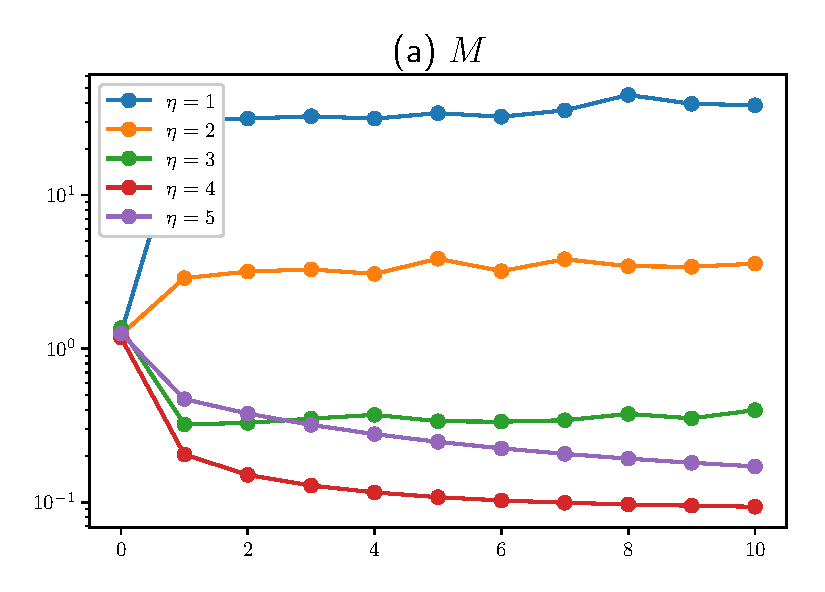
\includegraphics[width=0.95\linewidth]{figuras/RMch.eps}
		\end{subfigure}\hfill%
		\begin{subfigure}{.5\textwidth}
			\centering
			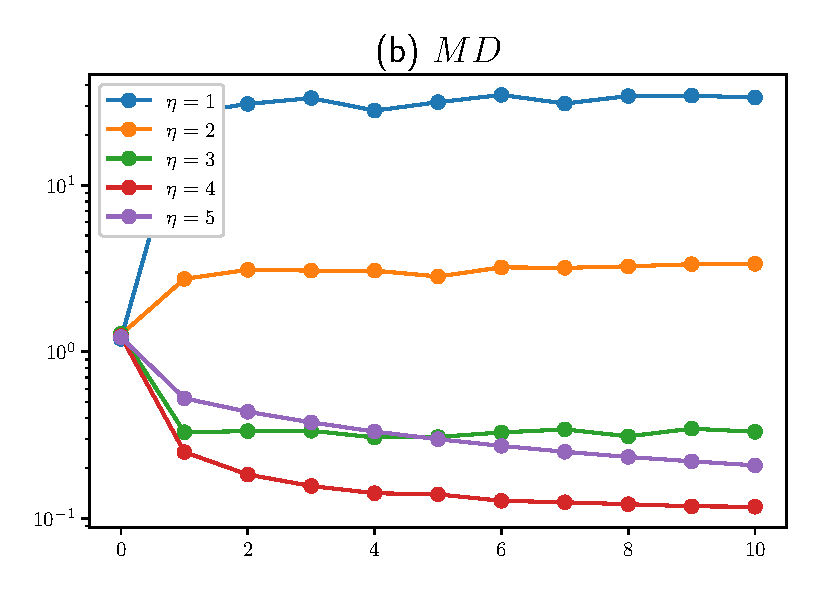
\includegraphics[width=0.95\linewidth]{figuras/RMchD.eps}
		\end{subfigure}\hfill%
		\newline
		\begin{subfigure}{.5\textwidth}
			\centering
			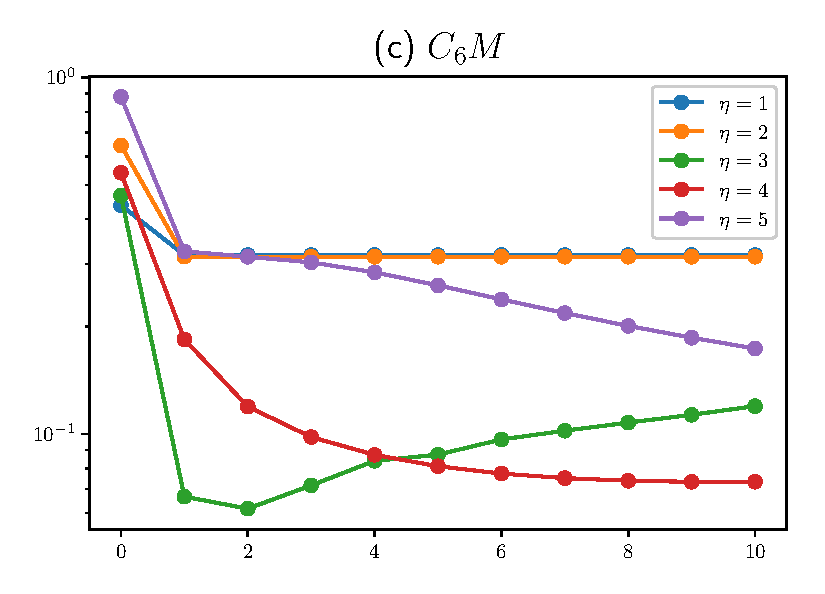
\includegraphics[width=0.95\linewidth]{figuras/C5o6RMch.eps}
		\end{subfigure}\hfill%
		\begin{subfigure}{.5\textwidth}
			\centering
			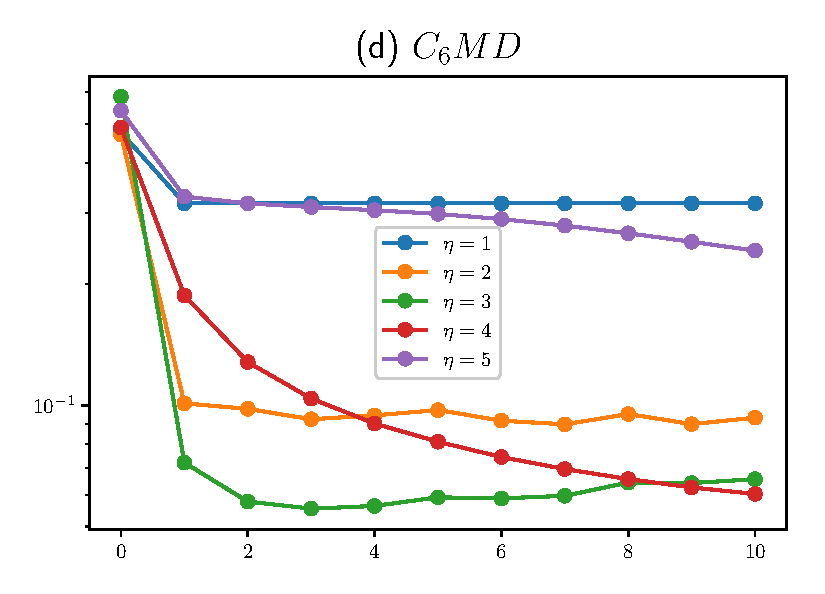
\includegraphics[width=0.95\linewidth]{figuras/C5o6RMchD.eps}
		\end{subfigure}\hfill%
		\newline\hspace*{-0.2cm}\makebox[0cm]{\rotatebox{90}{\hspace*{2.5cm}$log \left(  J^{(D_{val})}  \right) $\hspace*{-2.5cm}}}\hspace*{0.2cm}%
		\begin{subfigure}{.5\textwidth}
			\centering
			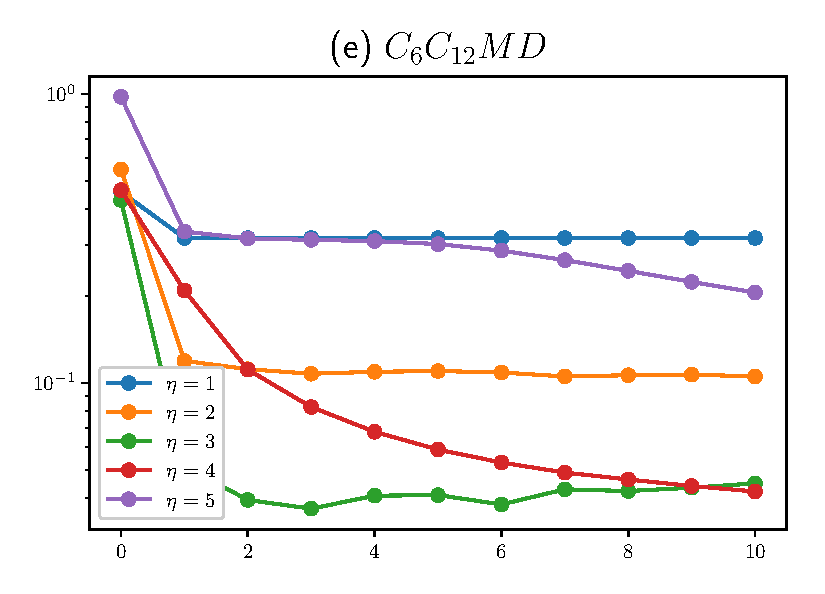
\includegraphics[width=0.95\linewidth]{figuras/C5o6C5o12RMchD.eps}
		\end{subfigure}\hfill%
		\begin{subfigure}{.5\textwidth}
			\centering
			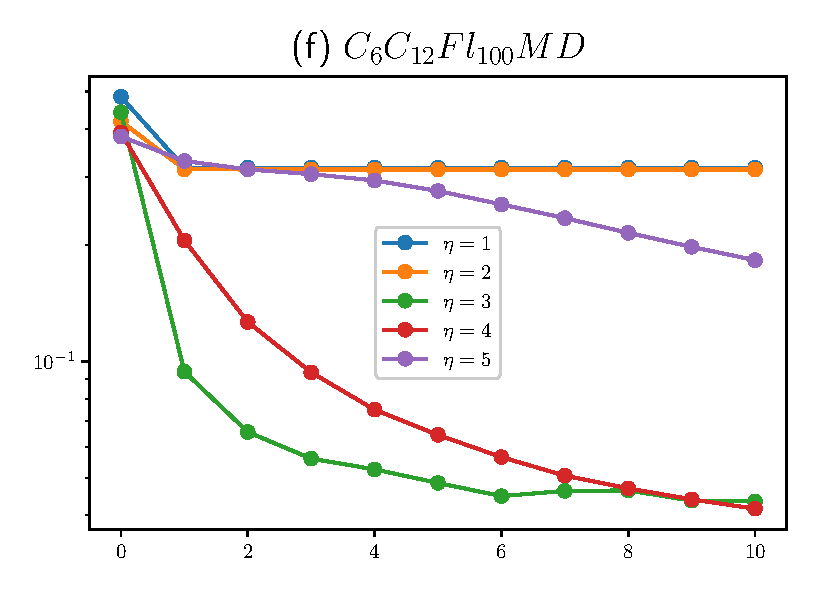
\includegraphics[width=0.95\linewidth]{figuras/C5o6C5o12Rfl100MchD.eps}
		\end{subfigure}
		\newline
		\begin{subfigure}{.5\textwidth}
			\centering
			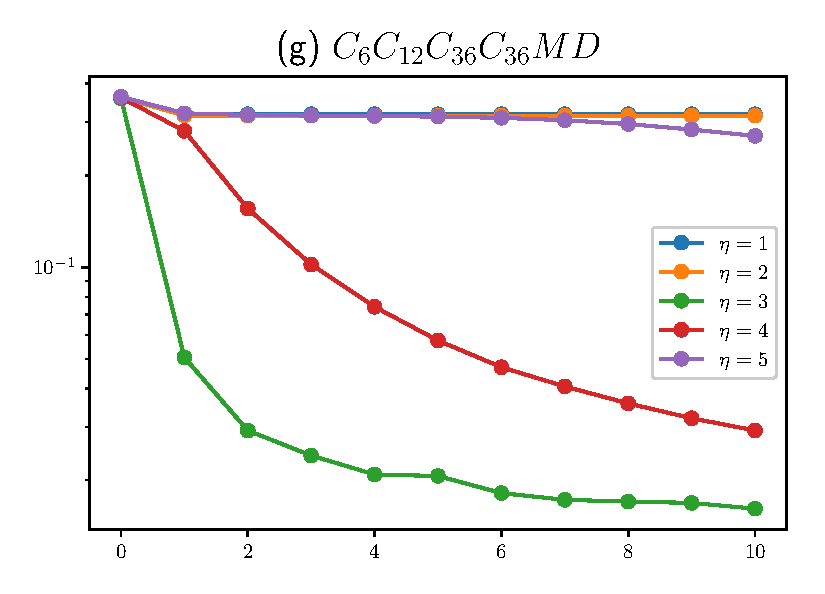
\includegraphics[width=0.95\linewidth]{figuras/C5o6C5o12C5o36C5o36RMchD.eps}
		\end{subfigure}\hfill%
		\begin{subfigure}{.5\textwidth}
			\centering
			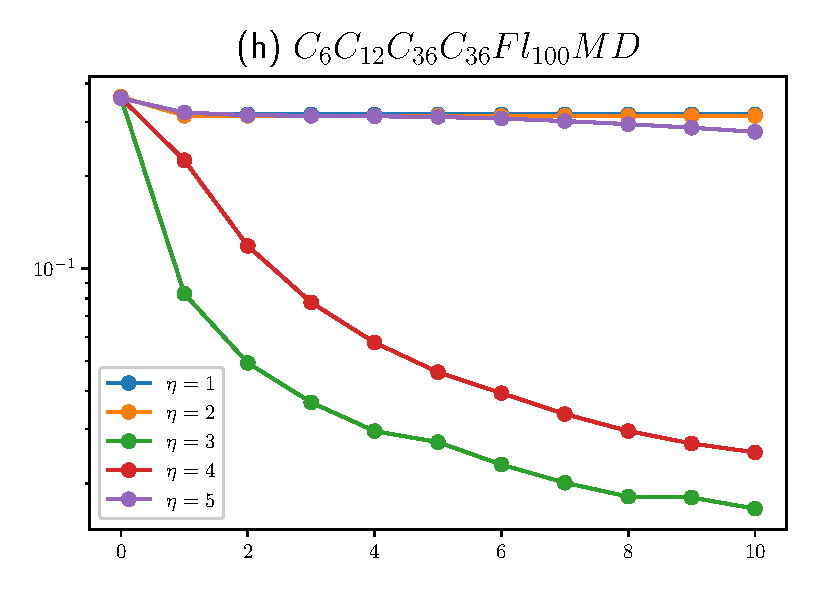
\includegraphics[width=0.95\linewidth]{figuras/C5o6C5o12C5o36C5o36Rfl100MchD.eps}
		\end{subfigure}\hfill%
		\newline
		$t$ (épocas)
	\end{center}
	\small Nos gráficos apresentamos a função custo na escala logarítmica de modo a facilitar a visualização. Os traços são apenas guias visuais. As arquiteturas estão indicadas nos títulos em correspondência com a tabela \ref{tab:modelos_iniciais} e os valores do hiper-parâmetro de aprendizado estão indicados na legenda.
\end{figure}

Na figura \ref{loss_val} podemos ver a evolução da função custo no conjunto de validação durante as 10 primeiras épocas para as arquiteturas na tabela \ref{tab:modelos_iniciais} e valores $\eta=1,2,3,4,5$. Para $\eta=1$ e $\eta=2$, vemos que o custo atinge um platô já durante as primeiras épocas da dinâmica. A estagnação em $J$ é um indicativo de que o gradiente da função de custo cresce de forma descontrolada. Quando isso ocorre, o algoritmo adaptativo Adam tende a privilegiar as atualizações em uma direção no espaço de $\{\mathbf{\Theta}\}$, anulando-as nas demais. Mais precisamente, antes das atualizações, o algoritmo normaliza $\nabla_{\mathbf{\Theta}} J$ pelo módulo do gradiente acumulado nos últimos lotes. Assim, se $|\nabla_{\mathbf{\Theta}} J| \rightarrow \infty$, $\Delta \mathbf{\Theta} \rightarrow 0$, exceto nas regiões onde o gradiente é proporcional ao seu momento. Em outras palavras, o algoritmo superestima o erro em uma determinada direção um detrimento das demais. Isso leva a rede a cometer os mesmos erros repetidamente nas direções não atualizadas. É importante ressaltar que quando esse fenômeno ocorre em algoritmos onde essa normalização não é aplicada (como o \textit{método do gradiente}, por exemplo), o gradiente e os parâmetros também crescem de forma descontrolada, evidenciado por uma divergência na função de custo. A dinâmica da função de custo nas redes $M$ e $MD$ corroboram para essa interpretação. No gráfico dessas arquiteturas podemos observar um aumento significativo no valor de $J$ antes das atualizações cessarem. Para uma análise mais precisa teríamos de acompanhar a evolução de $\mathbf{\Theta}$ ao longo do treino, o que esta fora do escopo do presente trabalho. No outro extremo, $\eta=5$, vemos um comportamento similar durante as épocas iniciais para algumas arquiteturas (c-h). Entretanto, a aparente estagnação nesses casos é devida à lenta convergência causada por esse valor do hiper-parâmetro. De fato, observamos uma melhoria no valor de $J$ na sequência da dinâmica. Desta forma, 
os valores $\eta=1, 2$ e $5$ apresentam comportamentos que devem ser evitados durante o treino, definindo, assim, os limites práticos para a busca do melhor hiper-parâmetro de aprendizado neste problema.

Dentro da região de interesse, o valor $\eta = 4$ exibe as dinâmicas mais estáveis, onde a função de custo apresenta um comportamento monotonicamente decrescente durante toda dinâmica, eventualmente estagnando, como visto em (a-d). Para as demais redes (d-h) percebemos que o valor da função de custo ainda apresentaria melhoras caso continuássemos a evolução por mais épocas. Para $\eta = 3$, vemos que a dinâmica é, de fato, mais rápida nas arquiteturas (c-h). Contudo, esse valor leva a instabilidades e, eventualmente, pioras no valor da função de custo (visto de (a) a (f) e mais acentuadamente em (c)). Esse fenômeno de overfitting foi discutido previamente no capítulo \ref{cap:neurais}. Nestes casos, o comportamento pode ser explicado por uma possível memorização dos exemplos de treino, ou seja, esse valor do hiper-parâmetro tende a superestimar os erros cometidos em casos específicos, levando à um cenário de coadaptação. Concluímos, então, que os valores $l_r=10^{-3}$ e $10^{-4}$ são os que apresentam o melhor compromisso entre velocidade de treino e estabilidade, respectivamente. Em seguida, analisaremos de forma mais detalhada essas configurações. 

\begin{table}[ht]
	\begin{center}
		\caption{Comparação entre as arquiteturas na décima época.}
		\label{tab:dinamica_inicial}
		\begin{tabular}{ |c|c|c|c|c|c|c| }
			\hline
			\multirow{2}{*}{modelo} & 
			\multirow{2}{*}{$l_r$} & 
			\multicolumn{2}{c|}{$D_{tr}$} &
			\multicolumn{2}{c|}{$D_{val}$} &
			\multirow{2}{*}{$\frac{J^{(D_{val})}}{J^{(D_{tr})}} - 1$}   \\ \cline{3-6}
			&  & $J$ & $\hat{p}_u$ & $J$ & $\hat{p}_u$  &  \\[2pt]
			% RMch
			\hline\hline
			\multirow{2}{*}{(a) $M$}
			& $10^{-3}$ & $1.81\,10^{-1}$ & $0.37$ & $3.98\,10^{-1}$ & $0.21$ & $1.20$ \\ \cline{2-7}
			& $10^{-4}$ & $4.77\,10^{-2}$ & $0.53$ & $9.34\,10^{-2}$ & $0.30$ & $0.96$ \\ \cline{2-7}
			
			% RMchD
			\hline\hline
			\multirow{2}{*}{(b) $MD$}
			& $10^{-3}$ & $1.50\,10^{-1}$ & $0.44$ & $3.31\,10^{-1}$ & $0.26$ & $1.20$ \\ \cline{2-7}
			& $10^{-4}$ & $7.59\,10^{-2}$ & $0.49$ & $1.17\,10^{-1}$ & $0.35$ & $0.55$ \\ \cline{2-7}
			
			% C5o6RMch
			\hline\hline
			\multirow{2}{*}{(c) $C_6M$}
			& $10^{-3}$ & $2.88\,10^{-3}$ & $\mathbf{0.96}$ & $1.20\,10^{-1}$ & $0.49$ & $40.49$ \\ \cline{2-7}
			& $10^{-4}$ & $2.41\,10^{-2}$ & $0.74$ & $7.34\,10^{-2}$ & $0.41$ & $2.05$ \\ \cline{2-7}
			
			% C5o6RMchD
			\hline\hline
			\multirow{2}{*}{(d) $C_6MD$}
			& $10^{-3}$ & $2.80\,10^{-3}$ & $\mathbf{0.96}$ & $6.56\,10^{-2}$ & $0.56$ & $22.40$ \\ \cline{2-7}
			& $10^{-4}$ & $3.27\,10^{-2}$ & $0.72$ & $6.02\,10^{-2}$ & $0.51$ & $0.84$ \\ \cline{2-7}
			
			% C5o6C5o12RMchD
			\hline\hline
			\multirow{2}{*}{(e) $C_6C_{12}MD$}
			& $10^{-3}$ & $\mathbf{2.33\,10^{-3}}$ & $\mathbf{0.96}$ & $4.49\,10^{-2}$ & $0.68$ & $18.24$ \\ \cline{2-7}
			& $10^{-4}$ & $2.12\,10^{-2}$ & $0.81$ & $4.21\,10^{-2}$ & $0.65$ & $0.99$ \\ \cline{2-7}
			
			% C5o6C5o12Rfl100MchD
			\hline\hline
			\multirow{2}{*}{(f) $C_6C_{12}Fl_{100}MD$}
			& $10^{-3}$ & $1.99\,10^{-2}$ & $0.74$ & $4.34\,10^{-2}$ & $0.60$ & $1.18$ \\ \cline{2-7}
			& $10^{-4}$ & $2.10\,10^{-2}$ & $0.78$ & $4.16\,10^{-2}$ & $0.62$ & $0.98$ \\ \cline{2-7}
			
			% C5o6C5o12C5o36C5o36RMchD
			\hline\hline
			\multirow{2}{*}{(g) $C_6C_{12}C_{36}C_{36}MD$}
			& $10^{-3}$ & $6.93\,10^{-3}$ & $0.92$ & $\mathbf{1.61\,10^{-2}}$ & $\mathbf{0.86}$ & $1.33$ \\ \cline{2-7}
			& $10^{-4}$ & $2.32\,10^{-2}$ & $0.81$ & $2.91\,10^{-2}$ & $0.76$ & $\mathbf{0.25}$ \\ \cline{2-7}
			
			% C5o6C5o12C5o36C5o36Rfl100MchD
			\hline\hline
			\multirow{2}{*}{(h) $C_6C_{12}C_{36}C_{36}Fl_{100}MD$}
			& $10^{-3}$ & $1.06\,10^{-2}$ & $0.86$ & $1.66\,10^{-2}$ & $0.81$ & $0.57$ \\ \cline{2-7}
			& $10^{-4}$ & $1.81\,10^{-2}$ & $0.81$ & $2.52\,10^{-2}$ & $0.75$ & $0.40$ \\ \cline{2-7}
			%otaro
			\hline\hline
			Pinto\cite{otaro} & - & - & 0.95 & - & 0.77 &  - \\ \cline{2-7} \hline
		\end{tabular}\hfill%
	\end{center}
	\small A última linha foi reproduzida do trabalho em \cite{otaro} que utilizou uma rede equivalente à $C_{64}C_{128}C_{256}C_{512}MaxFl_{4096}MD$ e 25 épocas em nossa nomenclatura.
\end{table}

Para melhor visualizar os modelos treinados com esses valores de $l_r$ fixos, compilamos na tabela \ref{tab:dinamica_inicial} o valor da função de custo, a acurácia do modelo para os conjuntos de validação e treino e o valor relativo do custo entre esses dois conjunto, dado por $J^{(D_{val})}/J^{(D_{tr})} - 1$, para as arquiteturas na tabela \ref{tab:modelos_iniciais}. Todos os valores na tabela foram medidos na décima época de treino. Na última linha temos o valor reportado por Pinto\cite{otaro} para comparação. A partir da tabela, a análise do valor relativo do custo (última coluna) denuncia a ocorrência de \textit{overffiting} nos modelos (c), (d) e (e). De fato, estes foram os modelos que alcançaram a maior acurácia no conjunto de treino não apresentando, entretanto, uma performance expressiva no conjunto de validação. Comparando os pares (a)-(b) e (c)-(d) podemos ver que a adição de \textit{dropout} contribuiu de forma significativa para o controle da coadaptação dos parâmetros da rede. Comportamento semelhante foi observado em todas as comparações feitas entre modelos com e sem regularização (ver apêndice \ref{cap:apendiceA}). Nas redes treinadas com \textit{maxpooling}, notamos, em geral, puco impacto ou até mesmo degradação na acurácia dos modelos quando defrontados com seus análogos com agrupamento fixo (ver apêndice \ref{cap:apendiceA}). No geral, a adição de camadas convolucionais melhoraram o desempenho das redes ao mesmo tempo em que limitaram a quantidade de parâmetros a serem optimizados. Nos pares (e)-(f) e (g)-(h), vemos que a adição de uma camada totalmente conectada deteriorou o desempenho. Este é um indicativo de que a adição arbitrária de camadas não necessariamente se traduz em arquiteturas mais expressivas.

Na última linha da tabela temos a precisão reportada no estudo de referência. Através da comparação com as configurações de rede utilizados no referido trabalho, podemos demonstrar a importância do estudo comparativo no projeto de redes neurais. Fomos capazes de obter resultados muito mais expressivos utilizando menos exemplos e redes mais simples. Em particular, nosso melhor resultado nos experimentos foi obtido em uma rede com 150 vezes menos parâmetros e uma base de treino 9 vezes menor. No estudo de referência estão presentes também fortes indicativos de coadaptação nos parâmetros. A acurácia reportada pelo autor é $23\%$ maior no conjunto de treino do que no de  validação, a despeito da aplicação de regularização com norma $L_2$ e dropout de $50\%$, sendo esses forte indicativos de memorização da base de treino.

\section{Treino completo} \label{sec:completo}

Assim com descrito na seção \ref{sec:abordagem}, escolhemos uma das configurações propostas para realizar um treino completo. Vamos definir como critério de escolha a eficiência de representação alcançada pela arquitetura, isto é, escolher a configuração que consegue alcançar o menor custo esperado com o uso de menos parâmetros. A escolha é fundamentada em duas considerações: a \textit{Navalha de Occam} e a generalidade de uso. A primeira nos leva a preterir soluções mais simples em detrimento das mais complexas, traduzindo-se, neste caso, em uma preferência por arquitetura de menos parâmetros. A segunda vem da observação de que em diferentes arquiteturas computacionais a memória é usualmente um fator limitante. Em sistemas embarcados ou \textit{smartphones}, por exemplo, esse seria um fator determinante para a escolha. De outra forma, com esta escolha estamos definindo que uma acurácia um pouco menor e alguns milissegundos a mais para a classificação de um token são trocas aceitáveis. A partir da tabela \ref{tab:dinamica_inicial} vemos que as configurações (g) e (h) apresentam um valor muito similar no valor esperado da função de custo, sendo (h) a escolhida por possuir menos parâmetros.  Outros requisitos levariam a escolhas diferentes. Frisamos que é possível estimar de antemão o tempo máximo de treino multiplicando o número de épocas máximas pelo tempo médio por época na tabela \ref{tab:modelos_iniciais}.

O modelo $C_6C_{12}C_{36}C_{36}Fl_{100}MD$ foi treinado até a quinquagésima época e a dinâmica do custo e da acurácia (total e por caractere) podem ser vistas na figura \ref{fig:chosenModel}. Em (i) vemos que o custo, no intervalo de épocas estudado, é uma função decrescente no tempo, comprovando a eficácia do método utilizado para a escolha da taxa de aprendizado. Notamos ainda que a inclinação na curva para o custo sugere que o modelo continuaria apresentando ganhos de performance caso o treino fosse continuado, evidenciando a escolha de uma configuração com boa expressividade. Isso nos permitiria obter um modelo ainda mais preciso, caso fosse necessário. Ressaltamos que o treino atingiu o número máximo de épocas predefinido, sem atingir nenhum dos demais critérios de parada propostos, o que evidência um aprendizado consistente (a média móvel no conjunto de treino é sempre decrescente) e controlado (sem overfitting detectado no conjunto de validação), sendo assim um treino exitoso segundo os critérios definidos na seção \ref{sec:treio_validacao}. Em (ii) vemos que o acerto por token apresenta um comportamento inverso ao do custo esperado tanto no conjunto de treino quanto no de validação, sendo tão maior quanto menor for o erro esperado pelo modelo. 

Na última época, a acurácia por token foi de $96.06\%$, sendo o classificador para o primeiro caractere o que apresentou melhor  desempenho de acertos, com acurácia final de $99.98\%$ e o classificador para o quarto o que apresentou pior desempenho, com uma acurácia final de $97.78\%$. A comparação entre os gráficos (iii) e (iv) mostram que, assim como esperado, o acerto de cada classificador é tão maior quanto menor for o custo associado. Um detalhe interessante a ser notado é que os caractere mais difíceis de serem identificados se encontram no meio do token (terceiro e quarto caractere) enquanto o primeiro classificador apresenta a melhor performance desde o inicio do treino. Apesar de não haver nenhuma forma de provarmos isso no momento, acreditamos que isso seja devido à facilidade de segmentação dos caracteres nessas posições, sendo o terceiro e o quarto os mais difíceis e o primeiro o mais fácil (vide figura \ref{fig:imgcaptchas} no capítulo \ref{cap:metodologia}).

O tempo total de treino foi de aproximadamente 4 horas e 16 minutos (3 horas e 33 minutos se descontarmos a etapa de validação), o que está de acordo com a estimativa fornecida a partir do tempos médio calculado durante a fase de experimentação na tabela \ref{tab:modelos_iniciais}. Para efeito de comparação, os experimentos do tralho de referência foram realizados em uma máquina com processador Intel\textsuperscript{\textregistered} Xeon\texttrademark E5-2686v4 (\textit{Broadwell}) de oito núcleos com 61 gb memória RAM e placa de aceleração gráfica VIDIA\textsuperscript{\textregistered} K80 com 12 gb de memória, durando aproximadamente 1 hora 18 minutos. Apesar de não podermos realizar uma comparação direta entre esses tempos, é de se notar que o aprendizado do modelo escolhido na infraestrutura que dispomos foi apenas três vezes mais longo que o aprendizado no trabalho de referência, a despeito da gritante diferença de poder computacional. 

\begin{figure}[ht]
	\begin{center}
		\caption{Dinâmica da arquitetura  $C_6C_{12}C_{36}C_{36}Fl_{100}MD$.}\label{fig:chosenModel}
		\begin{subfigure}{.5\textwidth}
			\centering
			\hspace{-0.02\linewidth}%
			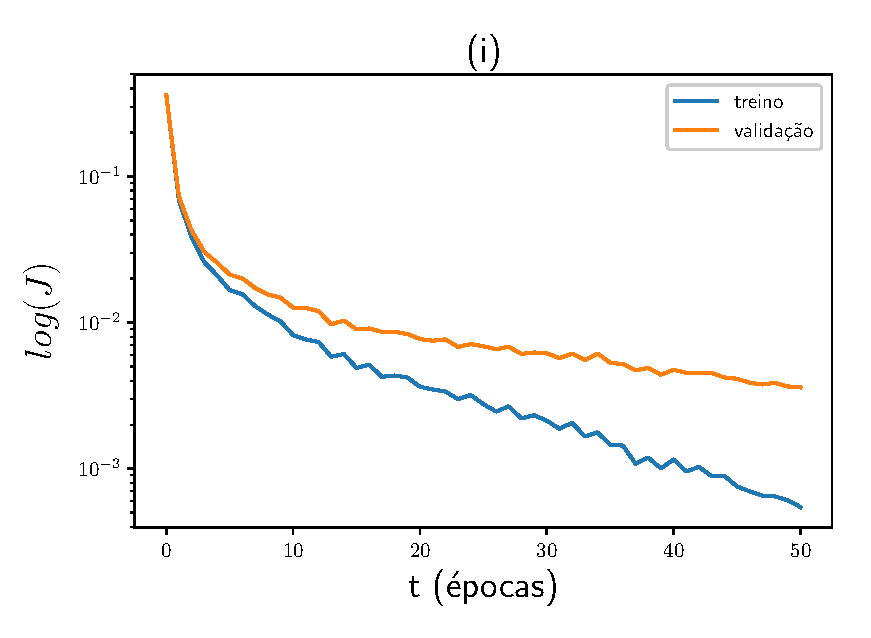
\includegraphics[width=0.98\linewidth]{figuras/C5o6C5o12C5o36C5o36Rfl100MchD_loss.eps}
		\end{subfigure}\hfill%
		\begin{subfigure}{.5\textwidth}
			\centering
			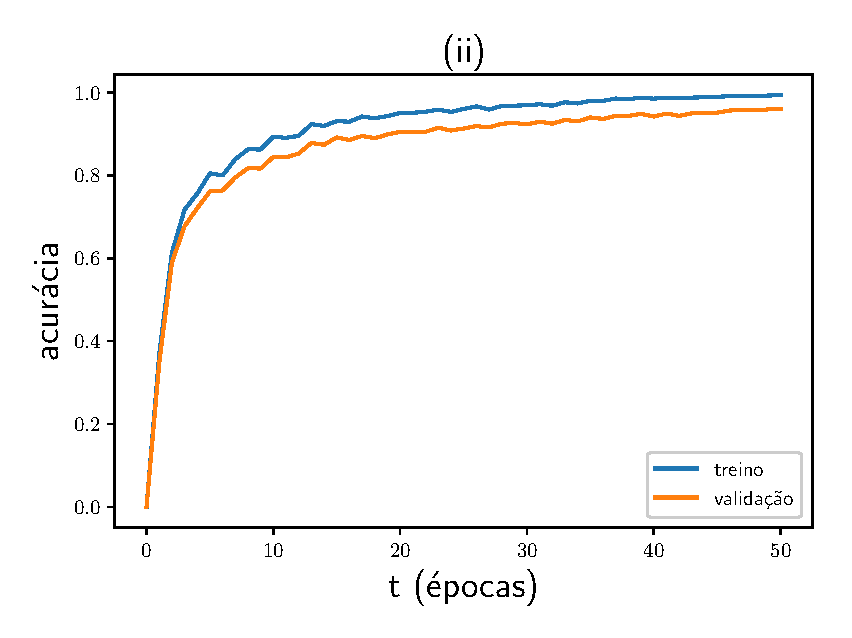
\includegraphics[width=0.95\linewidth]{figuras/C5o6C5o12C5o36C5o36Rfl100MchD_acc.eps}
		\end{subfigure}\hfill%
		\newline
		\begin{subfigure}{.5\textwidth}
			\centering
			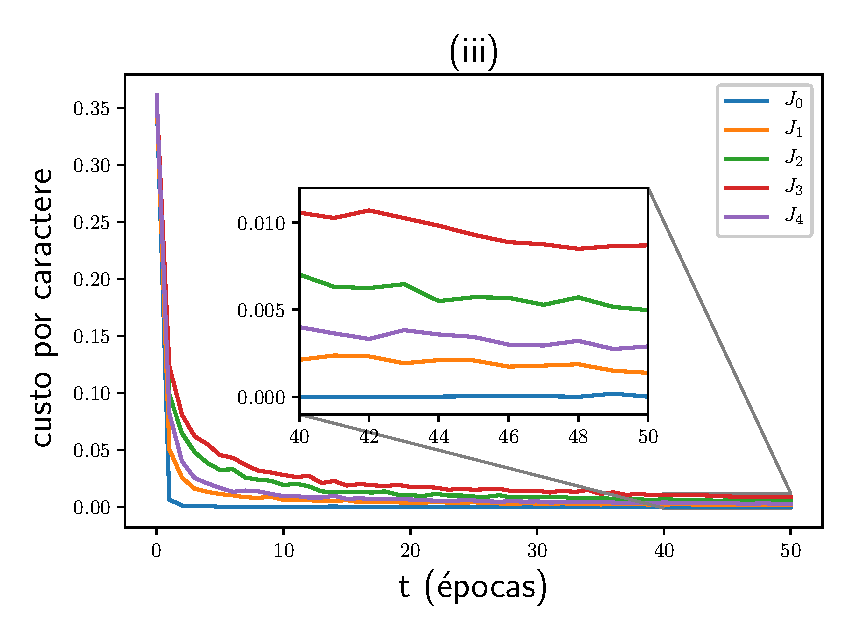
\includegraphics[width=0.95\linewidth]{figuras/C5o6C5o12C5o36C5o36Rfl100MchD_lossi.eps}
		\end{subfigure}\hfill%
		\begin{subfigure}{.5\textwidth}
			\centering
			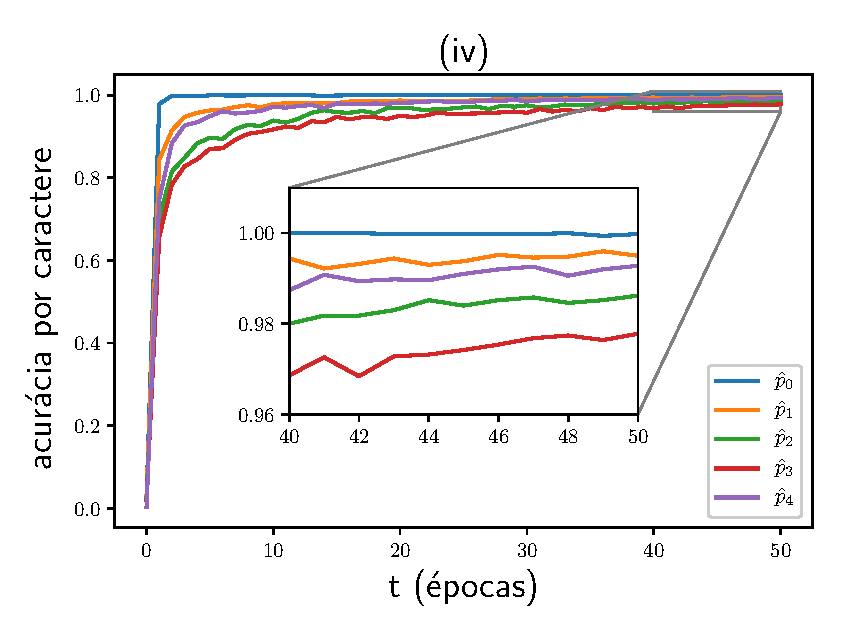
\includegraphics[width=0.95\linewidth]{figuras/C5o6C5o12C5o36C5o36Rfl100MchD_acci.eps}
		\end{subfigure}\hfill%
		\newline
	\end{center}
	\small (i) custo (escala logarítmica) e (ii) acurácia ao longo das épocas para o conjunto de treino e validação. (iii) custo e (iv) acurácia por classificador ao longo das épocas para o conjunto de validação.  
\end{figure}
 
\section{Discussão do Método}

O uso da metodologia proposta mostrou-se eficaz na construção de uma experimentação diversificada de configurações, abrangendo comportamentos substancialmente distintos entre sí. Essa diversidade foi o que permitiu fundamentar a escolha de uma arquitetura final baseando-se em critérios sólidos, possíveis devido ao pressuposto de comparação no qual o método se baseia. A configuração escolhida, de fato, demonstrou acurácia superior e maior eficiência de representação (menos parâmetros) do que os resultados do estudo escolhido como referência, demonstrando que a adição arbitrária de camadas não necessariamente se traduz em maior poder de expressividade. O resultado também corrobora o pressuposto de que a dinâmica inicial é informativa sobre o comportamento da rede durante o treino subsequente.

A partir dos experimentos realizados, podemos desenhar as observações que seguem. Arquiteturas convolucionais mostraram-se extremamente eficazes para o problema. Fixadas as demais configurações de rede, novas camadas convolucionais tendem à produzir modelos mais expressivos. De fato, esse tipo de camada tem sido aplicada com sucesso em diversos problemas de processamento de imagem. O compartilhamento de parâmetros nessas camadas ao mesmo tempo reduz o tamanho das arquiteturas e adiciona maior poder de expressão aos modelos. Camadas densas mostraram-se eficazes na redução das representações utilizadas no espaço de características, mas devem ser usadas de forma cautelosa. O \textit{dropout} mostrou-se uma ferramenta eficaz e computacionalmente barata para combater o \textit{overfitting}, melhorando a performance dos modelos estudados sem degradação significativa no tempo de computação. A operação de agrupamento com valor fixo apresentou tempo de execução menor do que a de \textit{maxout}, sem grandes diferenças de performance. Comportamentos substancialmente diferentes foram observados a partir da variação da taxa de aprendizado, indo da divergência das redes (altos valores) até a estagnação do aprendizado (baixos valores). Diferentes arquiteturas possuem requisitos próprios e alcançam performances distintas.

Em resumo, o método proposto nos permitiu escolher de forma embasada uma configuração de rede que atendesse aos requisitos impostos e ainda apresentasse uma boa performance. Adicionalmente, a análise comparativa nos fornece informações cruciais para a construções se novas configurações e refinamento dos resultados para o problema estudado.  